\documentclass[11pt]{article}
\usepackage[T1]{fontenc}
\usepackage[utf8]{inputenc}
\usepackage{lmodern}
\usepackage[letterpaper,margin=1in]{geometry}
\usepackage{amsmath,amssymb,amsthm,mathtools}
\usepackage{booktabs,longtable,tabularx,array,enumitem,microtype}
\usepackage{xcolor}
\usepackage{tikz}
\usetikzlibrary{arrows.meta,positioning,fit,backgrounds}
\usepackage[hidelinks]{hyperref}

\hypersetup{
  pdftitle={A Conceptual Guide to Global SU(2) Heat-Kernel Action Enclosures},
  pdfauthor={Anonymous author},
  pdfsubject={Geometry, diffusion, lattice gauge theory, and derivative bounds}
}

\definecolor{deepblue}{RGB}{31,78,121}
\definecolor{softblue}{RGB}{222,235,247}
\definecolor{softgreen}{RGB}{226,239,218}
\definecolor{softorange}{RGB}{252,228,214}
\definecolor{softgray}{RGB}{242,242,242}
\definecolor{deepgreen}{RGB}{56,118,29}

\newtheorem{principle}{Guiding principle}[section]
\newtheorem{example}[principle]{Example}
\theoremstyle{definition}
\newtheorem{definition}[principle]{Definition}
\newtheorem{remark}[principle]{Remark}

\newcommand{\SU}{\mathrm{SU}(2)}
\newcommand{\dd}{\,\mathrm{d}}
\newcommand{\R}{\mathbb{R}}
\newcommand{\N}{\mathbb{N}}
\newcommand{\abs}[1]{\left|#1\right|}
\newcommand{\norm}[1]{\left\lVert#1\right\rVert}
\newcommand{\Tr}{\operatorname{Tr}}
\newcommand{\e}{\mathrm{e}}

\newcommand{\conceptbox}[2]{%
  \begin{center}
  \fcolorbox{deepblue}{softblue}{%
    \parbox{0.91\textwidth}{\textbf{#1}\par\smallskip #2}}
  \end{center}}

\title{A Conceptual Guide to Global $\SU$ Heat-Kernel Action Enclosures\\
\large Geometry, diffusion, lattice gauge theory, and why derivative bounds matter}
\author{Anonymous author}
\date{}

\begin{document}
\maketitle

\begin{abstract}
This document is a pedagogical companion to the paper
\emph{Global Arbitrary-Order Enclosures for the $\SU$ Heat-Kernel Action}.
It is written for a first-year PhD student who knows basic quantum field
theory or differential geometry but has not yet worked with compact-group
heat kernels.  The central object is the negative logarithm of the heat
kernel on $\SU$, used as a one-plaquette action in lattice gauge theory.

The guide develops the complete conceptual chain.  A continuum gauge field
produces link holonomies; their ordered product around a plaquette is an
element of $\SU$; conjugation reduces that element to a class angle; diffusion
on the group supplies a normalized probability density; and its negative
logarithm supplies an action.  Two exact representations of the heat kernel
then reveal complementary structures: the character expansion makes
normalization and convolution transparent, while the Poisson-image formula
exhibits the short-time Gaussian.  Their apparent endpoint singularities
lead naturally to a three-chart analysis.  Near the antipode, a continuous
$S^2$ family of minimizing geodesics changes the short-time prefactor and the
Hessian behavior.  We explain why derivative bounds of arbitrary prescribed
order, positivity estimates, Haar-probability tails, and exact rational
validation are useful inputs for constructive and renormalization-group
analysis.  We also separate these local results from the further arguments
needed for a continuum Yang--Mills theory or a mass gap.
\end{abstract}

\tableofcontents

\section{The broader picture}

Yang--Mills theory describes gauge fields: geometrically, connections on
principal bundles; physically, the carriers of nonabelian interactions.  In
four Euclidean dimensions the formal continuum action is
\begin{equation}\label{expl:eq:continuum-action}
 S_{\mathrm{YM}}[A]
 =\frac{1}{4g_0^2}\int \sum_{a,\mu,\nu}
 F_{\mu\nu}^a(x)F_{\mu\nu}^a(x)\,\dd^4x,
\end{equation}
where $A$ is a gauge potential, $F$ is its curvature, and $g_0$ is a coupling
constant.  This compact formula conceals the main mathematical difficulty:
the desired quantum theory is an infinite-dimensional probability measure
modulo gauge symmetry, and the physically relevant infrared behavior is
strongly nonperturbative.

Lattice gauge theory replaces continuous space by a grid and the connection
by group-valued parallel transports on links.  This gives a finite-dimensional
regulated model.  The regulator does not solve the theory, but it makes the
basic objects honest integrals rather than formal functional integrals.
The smallest gauge-invariant observable on the lattice is the plaquette
holonomy, the ordered product of four link variables around an elementary
square.  A lattice action assigns an energetic cost to each plaquette
holonomy.

The heat-kernel action is one particularly natural choice.  Instead of
choosing an arbitrary class function on the gauge group, one uses the
negative logarithm of the group's diffusion kernel.  The semigroup property
of diffusion then mirrors the composition of scales.  This is why heat-kernel
actions have long been important in lattice gauge theory
\cite{MenottiOnofri1981,Manton1980,BitarDukeJadid1985}.

\begin{figure}[ht]
\centering
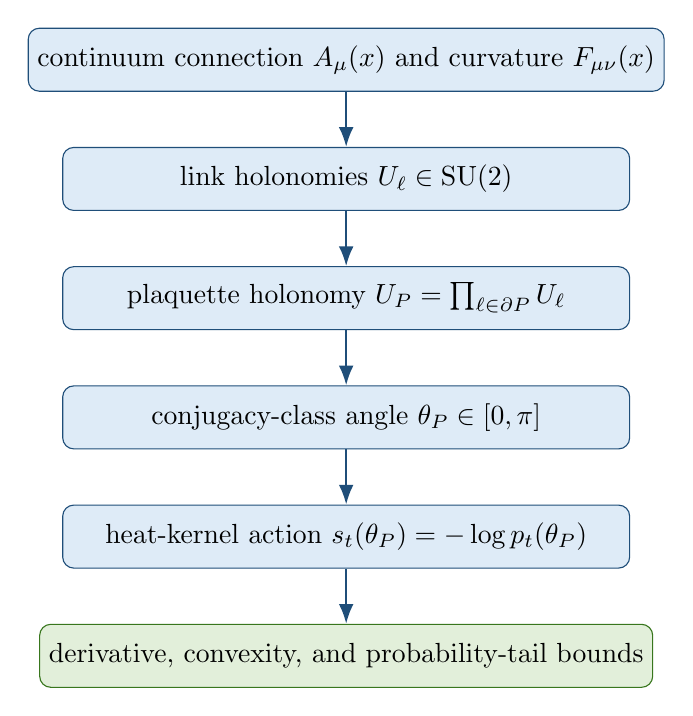
\begin{tikzpicture}[
  node distance=7mm,
  box/.style={draw=deepblue, rounded corners, fill=softblue,
              align=center, minimum width=7.2cm, minimum height=8mm},
  arr/.style={-{Latex[length=2.5mm]}, thick, deepblue}
]
\node[box] (A) {continuum connection $A_\mu(x)$ and curvature $F_{\mu\nu}(x)$};
\node[box,below=of A] (U) {link holonomies $U_\ell\in\SU$};
\node[box,below=of U] (P) {plaquette holonomy $U_P=\prod_{\ell\in\partial P}U_\ell$};
\node[box,below=of P] (theta) {conjugacy-class angle $\theta_P\in[0,\pi]$};
\node[box,below=of theta] (heat) {heat-kernel action $s_t(\theta_P)=-\log p_t(\theta_P)$};
\node[box,below=of heat,fill=softgreen,draw=deepgreen] (bounds)
 {derivative, convexity, and probability-tail bounds};
\draw[arr] (A)--(U);
\draw[arr] (U)--(P);
\draw[arr] (P)--(theta);
\draw[arr] (theta)--(heat);
\draw[arr] (heat)--(bounds);
\end{tikzpicture}
\caption{The chain from continuum gauge geometry to the quantitative object
studied in the paper.  Each arrow introduces a convention that must be fixed
before numerical constants can be compared.}
\label{expl:fig:chain}
\end{figure}

The paper addresses one link in this much longer chain: once the one-plaquette
heat-kernel action has been chosen, can we bound its derivatives explicitly,
at any requested finite order, across the entire compact group?  This is a
local and finite-dimensional question, but it is the kind of input required
before one can control nonlinear changes of variables, Taylor remainders, or
renormalization steps.

\conceptbox{The central question}{
For the exactly normalized heat kernel on $\SU$, how can one obtain explicit
finite-time bounds for derivatives of $s_t=-\log p_t$ from the identity all
the way to the cut locus, without hiding singular denominators or relying
only on asymptotic notation?}

\section{Minimum gauge-theory background}

\subsection{Connections, holonomy, and gauge invariance}

A gauge potential $A_\mu(x)$ is locally a Lie-algebra-valued one-form.  Given
a path $\gamma$, parallel transport along the path produces a group element
\[
 U_\gamma=\mathcal P\exp\left(i\int_\gamma A\right),
\]
where $\mathcal P$ orders noncommuting factors along the path.  Under a gauge
transformation, an open-path holonomy transforms at its endpoints.  The
holonomy around a closed loop transforms by conjugation, so its trace and
conjugacy class are gauge invariant.

On a hypercubic lattice, the fundamental variables are link matrices
$U_{x,\mu}\in\SU$.  For an elementary plaquette in the $\mu\nu$ plane,
\begin{equation}\label{expl:eq:plaquette}
 U_{P}=U_{x,\mu}U_{x+\hat\mu,\nu}
 U_{x+\hat\nu,\mu}^{-1}U_{x,\nu}^{-1}.
\end{equation}
The total action is normally a sum of class functions of $U_P$.  The
one-plaquette analysis asks how one such class function behaves before the
plaquettes are coupled through their shared links.

\subsection{Why start with \texorpdfstring{$\SU$}{SU(2)}?}

$\SU$ is the smallest nonabelian compact Lie group.  It already contains
noncommuting gauge degrees of freedom, yet its geometry is unusually explicit:
as a Riemannian manifold with the standard bi-invariant metric, it is the unit
three-sphere $S^3$.

Using the Pauli matrices $\sigma^a$ and generators
$T^a=\sigma^a/2$, every group element can be written as
\begin{equation}\label{expl:eq:su2-param}
 U=\cos\theta\,\mathbf 1+i\sin\theta\,\widehat n\!\cdot\!\sigma
   =\exp\bigl(2i\theta\,\widehat n\!\cdot\!T\bigr),
 \qquad 0\le\theta\le\pi,
\end{equation}
for a unit vector $\widehat n\in S^2$.  Conjugation rotates $\widehat n$ but
does not change $\theta$.  Consequently every central, or conjugation-invariant,
function depends only on the class angle $\theta$.

The basic identities are
\begin{equation}\label{expl:eq:trace-angle}
 \frac12\Tr U=\cos\theta,
 \qquad d(\mathbf 1,U)=\theta,
 \qquad \abs{X}=2\theta
 \quad\text{if }U=\exp(iX^aT^a).
\end{equation}
The final equality is an important convention warning: the norm of the
physics Lie-algebra coordinate $X$ is twice the geodesic class angle used in
the heat-kernel formulas.

Normalized Haar probability reduces on central functions to
\begin{equation}\label{expl:eq:haar}
 \int_{\SU}f(U)\,\dd H(U)
 =\frac{2}{\pi}\int_0^\pi f(\theta)\sin^2\theta\,\dd\theta.
\end{equation}
The factor $\sin^2\theta$ is the radial volume element of $S^3$.  It vanishes
at both endpoints because the two-sphere of angular directions collapses at
the identity and at the antipode.

\begin{definition}[Class angle]
The class angle $\theta\in[0,\pi]$ is the unique number satisfying
$\tfrac12\Tr U=\cos\theta$.  It is a coordinate on the space of conjugacy
classes, not a global coordinate system on the three-dimensional group.
\end{definition}

\section{Heat kernels: diffusion made geometric}

\subsection{From Euclidean diffusion to a compact group}

In flat $d$-dimensional Euclidean space, the heat equation
$\partial_tu=\tfrac12\Delta u$ has fundamental solution
\begin{equation}\label{expl:eq:euclidean-heat}
 k_t(x,y)=(2\pi t)^{-d/2}
 \exp\left[-\frac{|x-y|^2}{2t}\right].
\end{equation}
It is simultaneously a diffusion transition density and a normalized
Gaussian.  On a Riemannian manifold, the heat kernel $p_t(x,y)$ plays the
same role, but curvature, topology, and multiple geodesics modify the flat
formula.

For a compact Lie group with a bi-invariant metric, the heat kernel starting
at the identity is central.  We write it as $p_t(U)$ or $p_t(\theta)$ and fix
the convention
\begin{equation}\label{expl:eq:heat-equation}
 \partial_t p_t=\frac12\Delta p_t,
 \qquad \lim_{t\downarrow0}p_t=\delta_{\mathbf 1},
 \qquad \int_{\SU}p_t\,\dd H=1.
\end{equation}
Here $t$ is heat time.  In the lattice application it is related to a bare
coupling, but it is not Lorentzian time and should not be interpreted as the
physical duration of a process.

The semigroup law is
\begin{equation}\label{expl:eq:semigroup}
 p_{t_1+t_2}(U)=\int_{\SU}p_{t_1}(UV^{-1})p_{t_2}(V)\,\dd H(V).
\end{equation}
It says that two successive diffusion steps compose by group convolution.
This exact scale-composition property is the structural attraction of the
heat-kernel action.

\subsection{Why take the negative logarithm?}

A probability weight in Euclidean field theory has the form $\e^{-S}$.  If a
single plaquette is weighted by $p_t(U_P)$, its action is therefore
\begin{equation}\label{expl:eq:action}
 s_t(U_P)=-\log p_t(U_P).
\end{equation}
Near the identity and at short heat time, the diffusion kernel is approximately
Gaussian in geodesic distance, so
\begin{equation}\label{expl:eq:gaussian-action}
 s_t(\theta)\approx\frac{\theta^2}{2t}+\text{curvature corrections}
 +\text{image corrections}+\text{constant}.
\end{equation}
Thus $s_t$ resembles the Manton geodesic action, with systematic compact-group
corrections.  Additive constants affect the partition function but not action
derivatives.

\begin{principle}[Probability and action viewpoints]
The heat kernel $p_t$ is the natural object for normalization, convolution,
and tail probabilities.  The action $s_t=-\log p_t$ is the natural object for
forces, Hessians, Taylor expansions, and convexity.  Passing from one to the
other is safe only after a strictly positive lower bound for $p_t$ has been
established.
\end{principle}

\section{Two exact formulas, two kinds of insight}

The same $\SU$ heat kernel admits two exact representations.  The entire
paper is driven by the fact that neither one is uniformly convenient in all
regimes.

\subsection{The character expansion}

Irreducible representations of $\SU$ are labelled by
$n\in\mathbb N_0$ or spin $j=n/2$.  The representation has dimension $n+1$,
character
\[
 \chi_n(\theta)=\frac{\sin((n+1)\theta)}{\sin\theta},
\]
and Laplacian eigenvalue $-n(n+2)$.  Spectral decomposition gives
\begin{equation}\label{expl:eq:character}
 p_t(\theta)=\sum_{n=0}^{\infty}(n+1)
 \e^{-n(n+2)t/2}\frac{\sin((n+1)\theta)}{\sin\theta}.
\end{equation}
This formula makes several facts immediate:
\begin{itemize}
\item the kernel is built from group representations;
\item integration against Haar probability removes every nontrivial character,
so normalization is exact;
\item large representations are exponentially damped at fixed positive $t$;
\item the convolution law follows from the multiplication of spectral weights.
\end{itemize}

In spin notation the weight is $\e^{-2t j(j+1)}$.  A source that writes the
weight as $\e^{-\tau C_2(j)}$ is therefore using $\tau=2t$ under the present
generator convention.

\subsection{The Poisson-image formula}

Poisson summation reorganizes the same kernel into a sum over radial images:
\begin{equation}\label{expl:eq:image}
 p_t(\theta)=C_t\frac{1}{\sin\theta}
 \sum_{k\in\mathbb Z}(\theta+2\pi k)
 \e^{-(\theta+2\pi k)^2/(2t)},
 \qquad
 C_t=\frac{\e^{t/2}\sqrt{2\pi}}{2t^{3/2}}.
\end{equation}
The $k=0$ term is the local Gaussian.  The $k\ne0$ terms encode the compact
topology through paths that wrap around the radial covering coordinate.
At small $t$, their Gaussian suppression makes the short-distance structure
visible with very few terms.

\begin{table}[ht]
\centering
\begin{tabularx}{\textwidth}{>{\bfseries}p{0.20\textwidth}XX}
\toprule
Representation & What it makes transparent & Where care is needed \\
\midrule
Character sum & Haar normalization, representation content, semigroup law,
moderate and large heat time & many spectral modes can be needed at very small
heat time \\
Poisson images & short-time Gaussian, exponentially small images, endpoint
pairing, explicit tail estimates & the factor $1/\sin\theta$ is singular term
by term at $0$ and $\pi$ \\
\bottomrule
\end{tabularx}
\caption{The two exact representations answer different questions.}
\label{expl:tab:representations}
\end{table}

The formulas are exactly equal, rather than two unrelated approximations.
This equality lets one choose the representation that best matches the
geometric regime.

\section{Why the endpoints are subtle}

\subsection{A removable singularity is still dangerous in a proof}

The factor $1/\sin\theta$ in \eqref{expl:eq:image} diverges at both endpoints.
The full heat kernel is smooth, so the divergence must cancel in the complete
numerator.  But a smooth final answer does not justify differentiating
singular pieces separately.  Truncation or interval bounds can destroy the
cancellation unless the relevant images are paired first.

Near the identity, pair the images at $+2\pi k$ and $-2\pi k$.  Factoring out
the zero image gives
\begin{equation}\label{expl:eq:factorization}
 p_t(\theta)=C_t\e^{-\theta^2/(2t)}
 \frac{\theta}{\sin\theta}\bigl(1+q_t(\theta)\bigr),
\end{equation}
where
\begin{equation}\label{expl:eq:q}
 q_t(\theta)=2\sum_{k\ge1}\e^{-(2\pi k)^2/(2t)}
 \left[
 \cosh\frac{2\pi k\theta}{t}
 -\frac{2\pi k}{\theta}\sinh\frac{2\pi k\theta}{t}
 \right].
\end{equation}
The quotient involving $\theta$ has an even Taylor expansion.  An integral
identity removes it before differentiation:
\begin{equation}\label{expl:eq:sinh-integral}
 \frac{a}{\theta}\sinh\frac{a\theta}{t}
 =\frac{a^2}{t}\int_0^1\cosh\frac{sa\theta}{t}\,\dd s.
\end{equation}
This is a small technical step with a large conceptual consequence: all
derivatives can now be bounded using one nonsingular expression.

Taking the logarithm of \eqref{expl:eq:factorization} yields the exact
decomposition
\begin{equation}\label{expl:eq:action-decomposition}
 s_t(\theta)=\frac{\theta^2}{2t}
 +\log\frac{\sin\theta}{\theta}
 -\log(1+q_t(\theta))-\log C_t.
\end{equation}
The four terms have distinct meanings:
\begin{enumerate}[label=(\roman*)]
\item $\theta^2/(2t)$ is the flat Gaussian action;
\item $\log(\sin\theta/\theta)$ is the local curvature or volume correction;
\item $-\log(1+q_t)$ is the compact-topology image correction;
\item $-\log C_t$ fixes normalization and disappears under spatial derivatives.
\end{enumerate}

\subsection{The antipode and the cut locus}

The antipode $\theta=\pi$ is geometrically different from the identity.  On
$S^3$, every unit tangent direction at the identity determines a length-$\pi$
geodesic ending at the antipode.  The minimizing geodesics therefore form an
$S^2$ family.

This statement must be separated from the one-dimensional image formula.
The two leading terms in that formula have radial arguments approaching
$+\pi$ and $-\pi$.  They are two affine-Weyl image terms, not two individual
geodesics.  Their paired limit nevertheless encodes the continuous geometric
degeneracy.

With $\phi=\pi-\theta$ and $b_j=(2j+1)\pi$, the paired numerator is
\begin{equation}\label{expl:eq:cut-pair}
 2\e^{-(b_j^2+\phi^2)/(2t)}
 \left[b_j\sinh\frac{b_j\phi}{t}
 -\phi\cosh\frac{b_j\phi}{t}\right].
\end{equation}
Pairing occurs before division by $\sin\phi$.  The exact endpoint sum is
\begin{equation}\label{expl:eq:antipode-sum}
 p_t(\pi)=2C_t\sum_{j\ge0}
 \e^{-(2j+1)^2\pi^2/(2t)}
 \left(\frac{(2j+1)^2\pi^2}{t}-1\right).
\end{equation}
Its leading term gives
\begin{equation}\label{expl:eq:antipode-asymptotic}
 p_t(\pi)\sim \e^{t/2}\sqrt{2\pi}\,\pi^2
 t^{-5/2}\e^{-\pi^2/(2t)}
 \qquad (t\downarrow0).
\end{equation}

Away from a cut locus, a three-dimensional heat kernel has the generic power
$t^{-3/2}$.  A clean two-dimensional family of minimizing geodesics adds an
extra $t^{-2/2}=t^{-1}$ enhancement, producing $t^{-5/2}$.  This is the
Morse--Bott mechanism.  General heat-kernel results explain this phenomenon
in much broader settings \cite{ChenLiWu2023,NeelSacchelli2025}; the $\SU$
image sum makes it completely explicit.

\conceptbox{Geometric lesson}{
The exponent $\exp[-d^2/(2t)]$ records the shortest geodesic distance.  The
power of $t$ records how fluctuations accumulate around the minimizing set.
At the antipode the distance is still $\pi$, but the set of minimizers is
two-dimensional, so the prefactor changes.}

\section{The three-chart strategy}

No single estimate is both simple and well conditioned across the whole
class interval.  The paper therefore uses a small atlas adapted to the
geometry:
\[
 [0,\rho]\quad\text{identity chart},\qquad
 [\rho,\pi-\delta]\quad\text{transition chart},\qquad
 [\pi-\delta,\pi]\quad\text{cut chart}.
\]

\begin{figure}[ht]
\centering
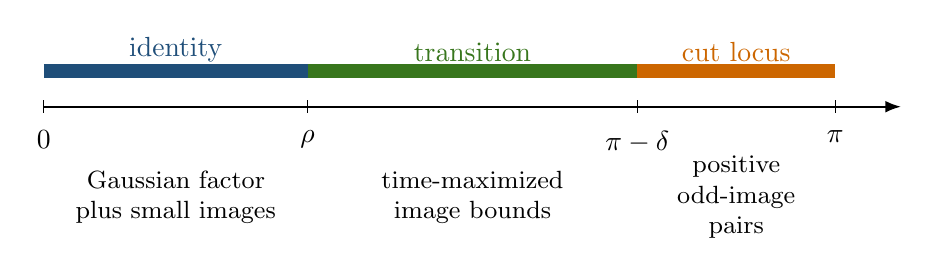
\begin{tikzpicture}[x=3.35cm,y=1cm]
\draw[thick,-{Latex[length=2mm]}] (0,0)--(3.25,0);
\draw (0,.08)--(0,-.08) node[below=3pt] {$0$};
\draw (1,.08)--(1,-.08) node[below=3pt] {$\rho$};
\draw (2.25,.08)--(2.25,-.08) node[below=3pt] {$\pi-\delta$};
\draw (3,.08)--(3,-.08) node[below=3pt] {$\pi$};
\draw[line width=5pt,deepblue] (0,.45)--(1,.45);
\node[above,deepblue] at (.5,.45) {identity};
\draw[line width=5pt,deepgreen] (1,.45)--(2.25,.45);
\node[above,deepgreen] at (1.625,.45) {transition};
\draw[line width=5pt,orange!80!black] (2.25,.45)--(3,.45);
\node[above,orange!80!black] at (2.625,.45) {cut locus};
\node[align=center,text width=2.9cm,font=\small] at (.5,-1.15)
 {Gaussian factor\\plus small images};
\node[align=center,text width=3.1cm,font=\small] at (1.625,-1.15)
 {time-maximized\\image bounds};
\node[align=center,text width=2.6cm,font=\small] at (2.625,-1.15)
 {positive odd-image\\pairs};
\end{tikzpicture}
\caption{A formula-adapted atlas on the conjugacy-class interval.}
\label{expl:fig:atlas}
\end{figure}

\subsection{Identity chart: perturbation of a Gaussian}

On $[0,\rho]$, the image correction $q_t$ in
\eqref{expl:eq:factorization} is exponentially small at short heat time.
For each derivative order $m$, the paper constructs a computable number
$Q_m$ such that
\begin{equation}\label{expl:eq:Q-bound}
 \sup_{0<t\le t_0}\sup_{0\le\theta\le\rho}
 \abs{q_t^{(m)}(\theta)}\le Q_m.
\end{equation}
The crucial zeroth-order condition is $Q_0<1$.  It implies
\begin{equation}\label{expl:eq:positive-floor}
 1+q_t(\theta)\ge1-Q_0>0,
\end{equation}
so the logarithm and its derivatives have a controlled denominator.

The curvature term has an independently convergent expansion from Euler's
product for the sine:
\begin{equation}\label{expl:eq:sine-series}
 \log\frac{\sin\theta}{\theta}
 =-\sum_{n\ge1}\frac{\zeta(2n)}{n\pi^{2n}}\theta^{2n},
 \qquad |\theta|<\pi.
\end{equation}
Thus the Gaussian, geometric, and image contributions are bounded separately
and then recombined.

\subsection{Transition chart: remove an artificial order restriction}

The simplest identity-chart bound replaces the heat-time dependence by its
value at $t_0$.  This is valid only when each exponential--polynomial factor
is monotone on $(0,t_0]$, and the condition becomes stricter as the derivative
order grows.

The transition chart instead maximizes the relevant function exactly:
\begin{equation}\label{expl:eq:H}
 \sup_{0<t\le t_0}\e^{-A/t}t^{-r}
 =\begin{cases}
 \e^{-A/t_0},&r=0,\\[2mm]
 \e^{-A/\tau_r}\tau_r^{-r},&r\ge1,
 \end{cases}
 \qquad \tau_r=\min\{t_0,A/r\}.
\end{equation}
This elementary optimization matters because spatial differentiation produces
powers of $t^{-1}$.  Handling the maximum exactly gives uniform finite-time
bounds without pretending the endpoint $t_0$ is always the worst case.

\subsection{Cut chart: bound the kernel before its logarithm}

Near $\pi$, the zero-image factorization is poorly conditioned because the
zero image is no longer the unique dominant geometric contribution.  The
paper instead works with the positive odd-image pairs
\eqref{expl:eq:cut-pair}.  It constructs
\begin{itemize}
\item derivative bounds $D_m^{\mathrm{cut}}(t,\delta)$ for $p_t$ itself;
\item a strictly positive principal-pair lower bound
$L_{\mathrm{cut}}(t,\delta)$ for $p_t$;
\item logarithmic derivative bounds obtained from the ratio of these
quantities.
\end{itemize}

The cut-chart constants necessarily depend on $t$.  This is not a weakness of
the estimate.  In fact, the antipodal action Hessian behaves as
\begin{equation}\label{expl:eq:antipode-hessian}
 s_t''(\pi)=-\frac{\pi^2}{3t^2}+O(t^{-1}),
\end{equation}
so no uniform $t\downarrow0$ Hessian bound can hold there.

\section{How derivative bounds pass through a logarithm}

Suppose a positive function has the form $f=1+q$ and we know bounds for
$q,q',\ldots,q^{(M)}$.  The first few derivatives illustrate the pattern:
\begin{align*}
 (\log f)'&=\frac{f'}{f},\\
 (\log f)''&=\frac{f''}{f}-\frac{(f')^2}{f^2},\\
 (\log f)'''&=\frac{f'''}{f}
 -3\frac{f'f''}{f^2}+2\frac{(f')^3}{f^3}.
\end{align*}
Every order contains a structured sum of products.  Writing each order by
hand is error prone.  Fa\`a di Bruno's formula organizes the result through
exponential partial Bell polynomials:
\begin{equation}\label{expl:eq:bell}
 \partial_\theta^m\log f
 =\sum_{\ell=1}^m(-1)^{\ell-1}(\ell-1)!
 \frac{\mathsf B_{m,\ell}(f',\ldots,f^{(m-\ell+1)})}{f^\ell}.
\end{equation}
If $f\ge L>0$ and $|f^{(j)}|\le D_j$, this immediately gives an explicit
upper bound at every requested finite order.

\begin{principle}[Why the zeroth-order bound comes first]
Derivative estimates for $p_t$ alone do not control derivatives of
$-\log p_t$.  One must first prove $p_t\ge L>0$ on the domain.  The lower
bound is the bridge between a heat-kernel estimate and an action estimate.
\end{principle}

\section{What ``arbitrary order'' means}

The result is arbitrary-order in an effective, finite sense.  Given any
chosen $M<\infty$, the construction outputs bounds through order $M$ together
with explicit convergent tails.  It does not assert that one fixed small-time
domain gives a uniform constant for all $M$ simultaneously.

This distinction is standard and important.  High derivatives introduce
large powers of $1/t$ and increasing combinatorial factors.  A statement
useful for computation or renormalization is therefore naturally organized
as
\[
 \text{choose }M
 \quad\longrightarrow\quad
 \text{choose a compatible domain}
 \quad\longrightarrow\quad
 \text{compute constants through order }M.
\]

Why might one need more than the Hessian?
\begin{enumerate}
\item The first derivative gives the local force in a variational or sampling
algorithm.
\item The Hessian gives convexity, stiffness, and Gaussian comparison.
\item Third and fourth derivatives control nonlinear Taylor remainders and
the leading corrections to a quadratic approximation.
\item Higher derivatives enter repeated changes of variables, cumulant
expansions, and multiscale effective actions.
\end{enumerate}

The value of the theorem is therefore not that every calculation will use
order eight or order twenty.  It is that the proof method does not have to be
redesigned when the required order changes.

\section{Hessian geometry and a concrete plaquette estimate}

For a radial function $f(\theta)$ on the unit three-sphere, the Hessian has
one radial and two tangential eigenvalues:
\begin{equation}\label{expl:eq:hessian-eigenvalues}
 \lambda_{\mathrm{rad}}=f''(\theta),
 \qquad
 \lambda_{\mathrm{tan}}=f'(\theta)\cot\theta
 \quad\text{with multiplicity two}.
\end{equation}
The factor $\cot\theta$ is geometric.  Tangential directions correspond to
changing the axis $\widehat n$ in \eqref{expl:eq:su2-param} while keeping the
radial class angle fixed to first order.

If
\[
 \abs{\partial_\theta^2(s_t-\theta^2/(2t))}\le R_2
 \quad\text{on }[0,\rho],
\]
then
\begin{equation}\label{expl:eq:convexity}
 \lambda_{\mathrm{rad}}(s_t)\ge t^{-1}-R_2,
 \qquad
 \lambda_{\mathrm{tan}}(s_t)
 \ge\rho\cot\rho\,t^{-1}-R_2.
\end{equation}
These inequalities express a simple physical picture: near the identity the
strong Gaussian curvature $1/t$ dominates the compact-geometry and image
corrections.

For the validated instance
\[
 t_0=\frac15,qquad \rho=1,qquad M=8,
\]
the paper obtains $R_2<0.455$.  Hence, for every $0<t\le1/5$ and
$0\le\theta\le1$,
\begin{equation}\label{expl:eq:numeric-convexity}
 \lambda_{\mathrm{rad}}(s_t)>4.545,
 \qquad
 \lambda_{\mathrm{tan}}(s_t)>2.755.
\end{equation}
At $t=1/5$, the scaled corrections also satisfy
\begin{equation}\label{expl:eq:scaled-remainders}
 tR_2<0.091,
 \qquad tR_3<0.058,
 \qquad tR_4<0.101.
\end{equation}

\begin{example}[Commuting radial plaquette path]
Consider
\[
 U_P(x)=\exp\bigl(2i(\theta+x)T^3\bigr).
\]
Its class angle is $\theta_P(x)=\theta+x$, so no noncommutative chain-rule
terms appear.  Equation \eqref{expl:eq:numeric-convexity} gives a second
derivative at least $4.545$ throughout the stated chart, while
\eqref{expl:eq:scaled-remainders} controls the third- and fourth-order
departure from the Gaussian action.  This is a concrete one-plaquette
coercivity statement.
\end{example}

For a general link variation, $\theta_P$ is a nonlinear function of several
noncommuting link matrices.  Then
\begin{equation}\label{expl:eq:chain-rule}
 \frac{\dd^2}{\dd x^2}s_t(\theta_P(x))
 =s_t''(\theta_P)(\theta_P')^2+s_t'(\theta_P)\theta_P''.
\end{equation}
The paper controls the derivatives of $s_t$; a full lattice estimate must
also control the derivatives of the plaquette map and sum the coupled
contributions in a specified norm.

\section{Connection with the weak-field continuum action}

For a smooth gauge field and lattice spacing $a$, the plaquette expansion has
the form
\begin{equation}\label{expl:eq:plaquette-expansion}
 X_P^a=a^2g_0F_{\mu\nu}^a(x)+O(a^3),
 \qquad U_P=\exp(iX_P^aT^a).
\end{equation}
Since $\theta_P=|X_P|/2$, the Gaussian part of the heat-kernel action gives
\begin{equation}\label{expl:eq:continuum-match}
 \frac{\theta_P^2}{2t}
 =\frac{a^4g_0^2}{8t}F_{\mu\nu}^aF_{\mu\nu}^a
 +O\left(\frac{a^5}{t}\right).
\end{equation}
Summing over plaquettes converts the factor $a^4$ into a Riemann sum for a
four-dimensional integral.  This explains how the lattice action can match
\eqref{expl:eq:continuum-action} after the convention-dependent relation
between $t$ and the bare coupling is fixed.

The next term in \eqref{expl:eq:action-decomposition} begins as
\[
 \log\frac{\sin\theta}{\theta}
 =-\frac{\theta^2}{6}+O(\theta^4).
\]
It is a compact-geometry correction without the leading $1/t$ enhancement.
The nonzero images are exponentially small on a fixed identity chart as
$t\downarrow0$.  Thus the local weak-field picture has a transparent
hierarchy:
\[
 \text{Gaussian continuum term}
 \quad+\quad
 \text{group-curvature correction}
 \quad+\quad
 \text{global image correction}.
\]

This matching is a necessary consistency check, but it is not by itself a
continuum-limit proof.  Such a proof must control the collective probability
measure as the number of lattice degrees of freedom diverges and the bare
parameters are tuned.

\section{Haar tails and the small-field/large-field split}

Let $\Pr_t$ be the probability measure on $\SU$ with density $p_t$ relative
to normalized Haar measure.  A tail probability
\[
 \Pr_t\{\theta\ge\rho\}
\]
measures how much of the one-plaquette heat-kernel distribution lies outside
the identity chart.

The exact normalization from the character formula avoids estimating a
denominator.  Combining the image formula with the Haar factor
$\sin^2\theta$ cancels one power of the apparent Weyl denominator.  The paper
obtains an explicit Gaussian-type upper bound whose dominant rate is
\begin{equation}\label{expl:eq:tail-rate}
 \log\Pr_t\{\theta\ge\rho\}
 \lesssim-\frac{\rho^2}{2t}
 \qquad (t\downarrow0,\ \rho<\pi).
\end{equation}

This is relevant to a common constructive strategy:
\begin{enumerate}
\item treat the small-field region using convexity and Taylor estimates;
\item show that the large-field region has sufficiently small probability;
\item prove that both controls survive the interaction between neighboring
degrees of freedom and successive scale transformations.
\end{enumerate}

The theorem supplies the one-variable tail in step 2.  In a four-dimensional
lattice measure, plaquettes share links and are not independent.  Therefore
the one-plaquette tail cannot simply be multiplied across plaquettes.  A
dependent-measure estimate remains necessary.

\section{Why exact rational validation is useful}

The analytic theorem produces convergent series and explicit formulas, but a
concrete parameter choice still involves many numerical comparisons: Is the
factor floor positive?  Is an omitted-tail ratio below one?  Is the Hessian
margin strictly positive after all upper bounds are combined?

The accompanying computation stores theorem-critical quantities as rational
numbers and decides strict inequalities using integers.  Floating-point
evaluation is reserved for a separate comparison of the character and image
formulas.  For the instance $t_0=1/5$, $\rho=1$, $\delta=1/5$, and $M=8$, the
record includes
\begin{itemize}
\item identity-chart image, logarithmic, and geometric bounds;
\item transition-chart bounds through order eight;
\item the cut-pair positivity margin;
\item normalized tail bounds;
\item radial and tangential plaquette Hessian margins.
\end{itemize}

This computational layer serves three purposes.  It prevents roundoff from
deciding a strict inequality, makes every numerical constant reproducible,
and catches normalization mistakes by comparing two exact formulas at sample
points including both endpoints.  It does not replace the analytic proof:
the code evaluates and checks a theorem whose inequalities are established in
the manuscript.

\section{Where this result sits in the Yang--Mills programme}

It is useful to distinguish levels of mathematical control.  The paper closes
the first highlighted level in the diagram below; the later levels require
new arguments.

\begin{figure}[ht]
\centering
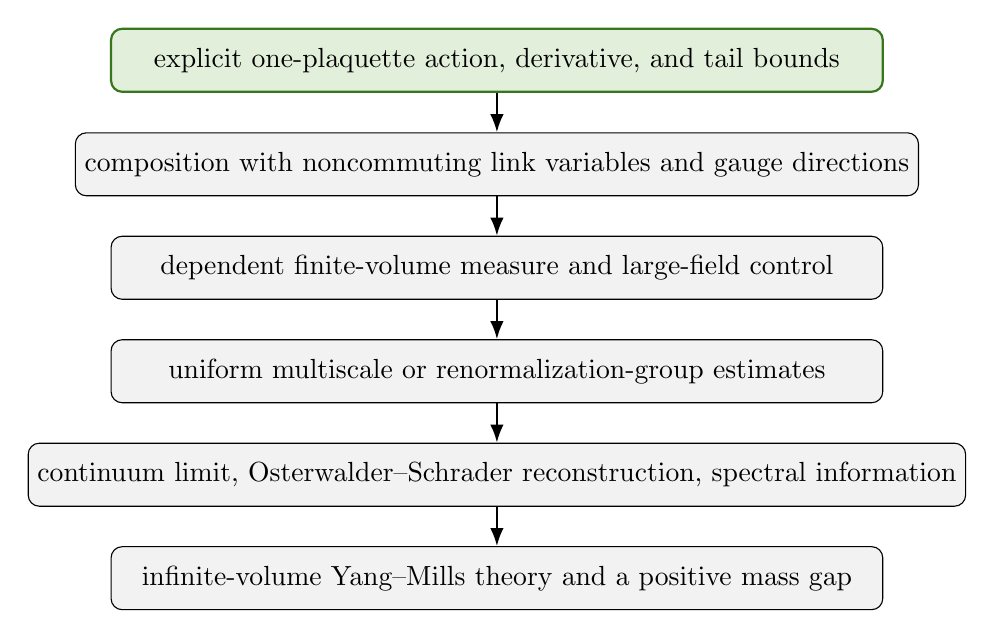
\begin{tikzpicture}[
  node distance=5mm,
  level/.style={draw,rounded corners,align=center,minimum width=9.8cm,
                minimum height=8mm,fill=softgray},
  done/.style={level,fill=softgreen,draw=deepgreen,line width=.8pt},
  arr/.style={-{Latex[length=2.3mm]},thick}
]
\node[done] (one) {explicit one-plaquette action, derivative, and tail bounds};
\node[level,below=of one] (link) {composition with noncommuting link variables and gauge directions};
\node[level,below=of link] (measure) {dependent finite-volume measure and large-field control};
\node[level,below=of measure] (rg) {uniform multiscale or renormalization-group estimates};
\node[level,below=of rg] (cont) {continuum limit, Osterwalder--Schrader reconstruction, spectral information};
\node[level,below=of cont] (gap) {infinite-volume Yang--Mills theory and a positive mass gap};
\draw[arr] (one)--(link);
\draw[arr] (link)--(measure);
\draw[arr] (measure)--(rg);
\draw[arr] (rg)--(cont);
\draw[arr] (cont)--(gap);
\end{tikzpicture}
\caption{A hierarchy of proof obligations.  The local result is useful because
later stages need quantitative microscopic input; it does not collapse the
later stages into consequences.}
\label{expl:fig:programme}
\end{figure}

The distinction prevents two opposite misunderstandings.
\begin{itemize}
\item The result is not a mass-gap proof.  It does not construct an
infinite-volume interacting measure, prove a continuum limit, or establish a
spectral gap for the reconstructed Hamiltonian.
\item Beyond the exact heat-kernel formula, the result supplies explicit
finite-time, arbitrary-finite-order control, including the cut locus, in a
form that can be inserted into later estimates.
\end{itemize}

The natural next mathematical questions are whether the one-plaquette bounds
can be transferred through the noncommutative plaquette map, whether a
small-field basin remains stable under block transformations, and whether
large-field probabilities can be controlled uniformly in volume.

\section{How to read the technical paper}

The main paper is easier to navigate once each section is associated with a
conceptual question.

\begin{longtable}{p{0.23\textwidth}p{0.69\textwidth}}
\toprule
Paper component & Question answered \\
\midrule
\endfirsthead
\toprule
Paper component & Question answered \\
\midrule
\endhead
Geometry and normalization & Which metric, generator, Haar measure, class
angle, trace, and physics-generator conventions define the constants? \\
Spectral and image formulas & Which two exact representations expose
normalization and short-time geometry? \\
Image hierarchy & How are paired nonzero images bounded through an arbitrary
chosen derivative order near the identity? \\
Action derivatives & How do those bounds pass safely through the logarithm,
and what do they imply for the Hessian? \\
Global atlas & How are the transition region and antipodal cut locus treated
without hiding endpoint singularities? \\
Haar tails & How much normalized heat-kernel mass lies outside the local
small-field chart? \\
Rational validation & Do the explicit parameter choices satisfy every strict
inequality using exact comparisons? \\
Lattice application & How do the group conventions match a plaquette
holonomy, and what concrete convexity margins result? \\
Appendices & Where are Poisson summation, image tails, Bell polynomials,
cut-pair bounds, and endpoint limits proved in detail? \\
\bottomrule
\end{longtable}

When checking the paper, it is useful to follow one dependency chain rather
than reading every formula in isolation:
\begin{equation}\label{expl:eq:dependency-chain}
\begin{aligned}
 \text{paired image formula}
 &\Longrightarrow \text{derivative bounds}
 \Longrightarrow \text{positive lower bound}\\
 &\Longrightarrow \text{logarithmic derivatives}
 \Longrightarrow \text{action Hessian and remainders}.
\end{aligned}
\end{equation}
The cut chart follows the same logic with $p_t$ itself in place of the factor
$1+q_t$.

\section{Conceptual glossary}

\begin{longtable}{p{0.22\textwidth}p{0.70\textwidth}}
\toprule
Term & Meaning in this work \\
\midrule
\endfirsthead
\toprule
Term & Meaning in this work \\
\midrule
\endhead
Class function & A function invariant under $U\mapsto VUV^{-1}$; on $\SU$ it
depends only on $\theta$. \\
Class angle & The number $\theta\in[0,\pi]$ determined by
$\tfrac12\Tr U=\cos\theta$. \\
Haar probability & The unique left- and right-invariant probability measure
on the compact group. \\
Heat kernel & The normalized transition density for Brownian diffusion
generated here by $\tfrac12\Delta$. \\
Heat-kernel action & The class function $s_t=-\log p_t$ used as a plaquette
action. \\
Character & The trace of a group representation; characters diagonalize
central convolution. \\
Poisson image & A Gaussian term in the resummed radial covering-space formula;
it is not an individual geodesic. \\
Weyl denominator & The factor $\sin\theta$ appearing in the radial character
and image formulas. \\
Cut locus & Points where minimizing geodesics cease to be unique or the
distance function loses smoothness; for the identity on $S^3$, the cut locus
is the antipode. \\
Morse--Bott family & A smooth positive-dimensional family of stationary or
minimizing configurations; here the $S^2$ family of antipodal geodesics. \\
Enclosure & An explicit lower or upper bound, often represented by rational
endpoints, that is guaranteed to contain the target quantity. \\
Positivity floor & A proved number $L>0$ such that the kernel or correction
factor is at least $L$ throughout a chart. \\
Arbitrary finite order & A method that produces bounds for every chosen
$M<\infty$, with constants and domain conditions allowed to depend on $M$. \\
Bell polynomial & A combinatorial polynomial organizing derivatives of a
composition such as $\log f$. \\
Plaquette & The smallest elementary loop on a lattice and the basic local
carrier of curvature. \\
Small-field chart & A neighborhood of the identity where the Gaussian action
dominates its compact-group corrections. \\
\bottomrule
\end{longtable}

\section{Takeaway}

The heat-kernel action sits at an instructive intersection of geometry,
probability, representation theory, and lattice gauge theory.  Its spectral
formula says that diffusion is organized by group representations.  Its image
formula says that short-time diffusion is locally Gaussian but globally aware
of compact topology.  Its logarithm turns probability into an action.  Its
endpoint behavior remembers the multiplicity of minimizing geodesics.

The technical achievement of the companion paper is to make these statements
quantitative on the full class interval.  Pairing removes false endpoint
singularities; chart-specific estimates respect the different identity and
cut-locus geometries; positivity bounds make logarithmic differentiation
legitimate; Bell polynomials extend the calculation to any prescribed finite
order; and rational validation turns the analytic estimates into reproducible
numerical instances.

For a new researcher, the most important perspective is one of scale and
scope.  The result provides a controlled microscopic action and a precise
small-field input.  The next frontier is to show that this local control
survives gauge coupling, large fields, volume growth, and repeated coarse
graining.  That is where the one-plaquette geometry becomes part of the wider
constructive Yang--Mills problem.

\bibliographystyle{alpha}
\bibliography{references}

\end{document}
